\documentclass[11pt]{article}
\usepackage[T1]{fontenc}
\usepackage[utf8]{inputenc}
\usepackage{lmodern,microtype,amsmath,amssymb,amsthm,mathtools}
\usepackage[a4paper,margin=27mm]{geometry}
\usepackage{xcolor,xurl,enumitem,booktabs,tikz}
\usetikzlibrary{arrows.meta}
\usepackage[unicode,colorlinks=true,linkcolor=blue!45!black,citecolor=green!35!black,urlcolor=blue!55!black]{hyperref}
\setlength{\emergencystretch}{2em}
\numberwithin{equation}{section}
\newtheorem{theorem}{Theorem}[section]
\newtheorem{proposition}[theorem]{Proposition}
\newtheorem{lemma}[theorem]{Lemma}
\newtheorem{corollary}[theorem]{Corollary}
\theoremstyle{definition}\newtheorem{definition}[theorem]{Definition}
\theoremstyle{remark}\newtheorem{remark}[theorem]{Remark}
\newcommand{\ii}{\mathrm i}
\newcommand{\Rea}{\operatorname{Re}}
\newcommand{\Loga}{\operatorname{Log}}
\newcommand{\calQ}{\mathcal Q}
\title{Holomorphic asymptotics of central shared face coefficients}
\author{}\date{}
\begin{document}\maketitle
\begin{abstract}
A marked spherical diagram gives an exact coefficient in shared face
variables. At each crossing region its finite Casimir polynomial has a
central degree part. We prove a nonzero holomorphic Gaussian expansion
for the coefficient obtained by selecting that part everywhere, and a
strict bound away from the complete spectral point. Both statements
hold through all integer levels and both parities, with the original
coefficient targets. The local proof starts from the actual cofactor
recurrence, including the odd skipped-row term. Positive finite matrices
control every other face phase, and the real spectral estimate is sewn
on one common radius vector. The resulting estimates supply the source
hypotheses of the oscillatory filling theorem. No estimate for the other
degree parts of the invariant, or independent identification with a
hyperbolic volume, is asserted.
\end{abstract}

\section{The coefficient and the theorem}
Let $\mathcal T$ be a finite simple oriented triangulation of the sphere.
A perfect matching of its dual pairs its triangles across $R$ edges.
Its $R+2$ vertices are called faces, following their role in the original
diagram. Choose a nonmatching edge $uv$ as the mark. The two face
variables $L_u,L_v$ are set to zero; the remaining $R$ variables are
ordinary. The order at a matched pair is $(x,b,c,y)$: its triangles
are $(x,b,y)$ and $(x,c,y)$, with their induced opposite orientations
along the matching edge $xy$. Repeated occurrences of a face always
denote the same variable.
In particular $x+y>0$ on the positive ordinary radii of every pair:
otherwise its matching edge would be the unique edge $uv$, which is
the nonmatching mark. Each pair also has a nonmonomial triangle.
If one outer face is protected, only one other zero remains, so at
least one middle is positive; if both outers are positive, both
triangles are nonmonomial.

Fix $N\ge3$ and write
\[
 d=N-1,\quad m=\lfloor N/2\rfloor,\quad J=\lfloor d/2\rfloor,
 \quad\theta=\pi/N,\quad s_j=2\sin(j\theta),
 \quad a_j=4\cos^2((j+\tfrac12)\theta).
\]
The polynomial operator on $1,z,\ldots,z^d$ is
\begin{equation}\label{sa:operator}
 \mathsf C z^j=2\cos((2j+1)\theta)z^j
             -s_j^2(x+y)z^{j-1}-s_js_{j-1}xy z^{j-2}.
\end{equation}
Absent terms vanish. For $\chi_N(t)=2T_N(t/2)+2$, let
\[
 V_N(\sigma;\mathsf C)
       =\frac{\chi_N(\sigma)-\chi_N(\mathsf C)}{\sigma-\mathsf C}.
\]
This is a polynomial divided difference. The finite Fourier theorem
\cite[Proposition 4.1]{Finite} identifies $\mathsf C$, after evaluation,
transpose and a diagonal gauge, with each $N$-dimensional residue block
of the physical pair Casimir. Thus its homogeneous polynomial
\[
 H_V(x,b,c,y;\sigma)=\sum_{0\le i\le j\le d}
                   V_N(\sigma;\mathsf C)_{ij}b^ic^{d-j}
\]
retains the original values and nilpotent normals. The central part
$H_{V,\mathrm C}$ keeps $i\le J$ and $d-j\le J$. The other two
parts keep $d-j>J$ or $i>J$; we do not estimate them here.

Put $\sigma_e=-2\cos(2\pi\delta_e)$ and define the raw central coefficient
\begin{equation}\label{sa:coefficient}
 C_N(\delta)=
 \left[\prod_{f\ne u,v}L_f^d\right]
 \left.\prod_{e=1}^R H_{V,\mathrm C}
       (L_{x_e},L_{b_e},L_{c_e},L_{y_e};\sigma_e)
                  \right|_{L_u=L_v=0}.
\end{equation}
This definition includes its sign $(-1)^{dR}$. Its identification as a
contribution to the original marked evaluation, with cups, caps and
framing still present, is the exact diagram theorem
\cite[Theorem 9.1 and Corollary 9.2]{Finite}. The coefficient itself is
the object of the present analytic theorem.

\begin{figure}[t]
\centering
% Native TikZ source. Incidence drawing, not a circle packing.
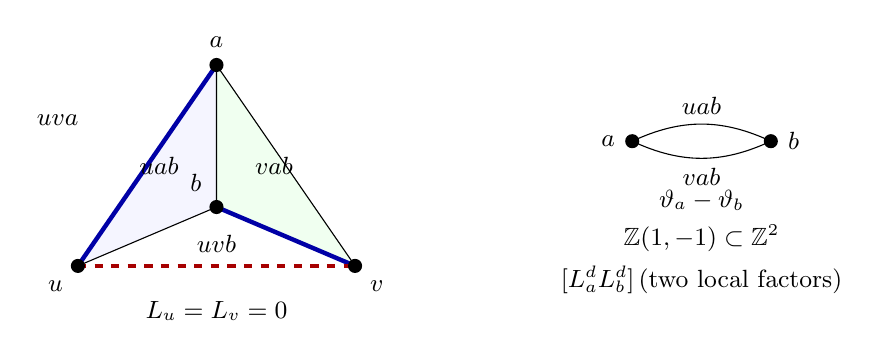
\begin{tikzpicture}[scale=.88, every node/.style={font=\small},
  vertex/.style={circle,fill=black,inner sep=1.8pt},
  matching/.style={draw=blue!65!black,line width=1.6pt},
  marked/.style={draw=red!65!black,dashed,line width=1.2pt}]
  \coordinate (u) at (-2,0);
  \coordinate (v) at (2,0);
  \coordinate (a) at (0,2.9);
  \coordinate (b) at (0,.85);
  \fill[blue!4] (u)--(a)--(b)--cycle;
  \fill[green!6] (v)--(a)--(b)--cycle;
  \draw[matching] (u)--(a);
  \draw[matching] (v)--(b);
  \draw[marked] (u)--(v);
  \draw (u)--(b)--(a)--(v);
  \node[vertex,label=below left:$u$] at (u) {};
  \node[vertex,label=below right:$v$] at (v) {};
  \node[vertex,label=above:$a$] at (a) {};
  \node[vertex,label=above left:$b$] at (b) {};
  \node at (-.83,1.45) {$uab$};
  \node at (.83,1.45) {$vab$};
  \node at (0,.32) {$uvb$};
  \node[anchor=east] at (-1.85,2.1) {$uva$};
  \node at (0,-.65) {$L_u=L_v=0$};
  \begin{scope}[xshift=7cm]
    \coordinate (aa) at (-1,1.8);
    \coordinate (bb) at (1,1.8);
    \draw (aa) to[bend left=25] node[above] {$uab$} (bb);
    \draw (aa) to[bend right=25] node[below] {$vab$} (bb);
    \node[vertex,label=left:$a$] at (aa) {};
    \node[vertex,label=right:$b$] at (bb) {};
    \node[align=center] at (0,.65)
      {$\vartheta_a-\vartheta_b$\\[3pt]$\mathbb Z(1,-1)\subset\mathbb Z^2$};
    \node at (0,-.2) {$[L_a^dL_b^d]\,(\text{two local factors})$};
  \end{scope}
\end{tikzpicture}

\caption{A combinatorial tetrahedral sphere and its ordinary phase graph.
The vertices $u,v,a,b$ name shared face variables. The marked edge $uv$
(red, dashed) sets $L_u=L_v=0$; the two blue matching edges are $ua$
and $vb$. The outer face of the planar drawing is the triangle $uva$.
The two triangles with two ordinary vertices, $uab$ and $vab$, compare the same
ordinary phases $\vartheta_a,\vartheta_b$, giving two copies of the
primitive difference row $(1,-1)$. Their coefficients add in the
Hessian, while the quotient angular measure remains
$d\vartheta_b/(2\pi)$ after $\vartheta_a=0$. The coefficient target is
$L_a^dL_b^d$, with each variable shared by the two local factors.
The drawing specifies incidence only; its lengths are not packing radii.}
\label{sa:shared-figure}
\end{figure}

Here is the sole positive-radius input. It can be supplied by the
complete packing of the marked triangulation, but is stated analytically
so that the theorem can be used without a geometric normalization.
For nonnegative $(w_1,w_2,w_3)\ne(0,0,0)$ define
\begin{align}
 \Lambda(t)&=-\int_0^t\log|2\sin v|\,dv,\notag\\
 e(a)&=\pi^{-1}\{\Lambda(\pi a)+\Lambda(\pi/2-\pi a)\},\notag\\
 \calQ(w)&=\max_{\substack{a_i\ge0,\ \sum a_i=1/2\\a_i=0\text{ if }w_i=0}}
             \sum_i\{e(a_i)+a_i\log w_i\}.\label{sa:entropy}
\end{align}
Terms on zero coordinates are omitted, and $e(0)=e(1/2)=0$.
Choose positive ordinary radii $\rho_f$ such that
\begin{equation}\label{sa:stationarity}
 \mathcal F(L)=\sum_{e=1}^R
     \{\calQ(x_e,b_e,y_e)+\calQ(x_e,c_e,y_e)\}
                         -\sum_{f\ne u,v}\log L_f
 \quad\text{is stationary at }L=\rho
\end{equation}
modulo common scale. Set $\Phi=\mathcal F(\rho)$.
Zeros remain exactly zero. The diagram and radii are fixed before $N$
tends to infinity.

\begin{theorem}[The actual central source]\label{sa:main}
Under these hypotheses there is a fixed complex polydisk about zero
and, for all sufficiently large $N$, holomorphic functions $A_N$ and
holomorphic $(R-1)$-by-$(R-1)$ matrices $H_N$ on it such that
\begin{equation}\label{sa:H1}
 C_N(\delta)=
 \frac{(-1)^{dR}N^{2R}e^{NA_N(\delta)}}
 {(2\pi N)^{(R-1)/2}\sqrt{\det H_N(\delta)}}
                         (1+O(N^{-1})).
\end{equation}
The relative error is holomorphic and uniform on smaller closed
polydisks. The square root continues the positive face Hessian at zero.
The actions are separately even and real on the real chart, and
$A_N\to A_0$, $H_N\to H_0$ locally uniformly with every fixed derivative.
The face Hessian $H_0(0)$ is positive definite. Moreover
\begin{equation}\label{sa:hessian}
 \begin{aligned}
 A_0(0)&=\Phi,\qquad A_0''(0)=-2\operatorname{diag}(\kappa_e),\\
 \kappa_e&=\frac{\pi\bigl(\sqrt{b_e(x_e+y_e)+x_ey_e}
                    +\sqrt{c_e(x_e+y_e)+x_ey_e}\bigr)}
                    {x_e+y_e}>0.
 \end{aligned}
\end{equation}
All face values in the last expression are at $\rho$.

For every $0<\eta<1/2$ there are $\gamma_\eta,\tau_\eta>0$ such that,
for all sufficiently large integer levels,
\begin{equation}\label{sa:H2}
 |C_N(x+\ii y)|\le e^{N(\Phi-\gamma_\eta)}
 \quad(x\in[-1/2,1/2]^R,\ \max_e|x_e|\ge\eta,
                       \ \max_e|y_e|\le\tau_\eta).
\end{equation}
Fixed derivatives have the corresponding bounds on smaller domains.
There is no prime-level restriction and no change of normalization
between even and odd levels.
\end{theorem}

We define the finite actions directly from the actual local polynomial.
They are not asserted to equal a separately constructed approximate
fold interpolation. In particular no value-only interpolation is
differentiated to obtain a normal.

\section{Finite cofactors and positive nodal matrices}\label{sa:finite}
Set $u(\delta)=-4\sin^2(\pi\delta)$, $A=x+y$, $P=xy$ and
$\alpha_j=a_j+u$. In this section $u$ is a spectral coordinate, not
the protected face. The cleared cofactor is the polynomial
\begin{equation}\label{sa:R}
 R_{-1}=0,\quad R_0=1,\qquad
 R_j=b^j\prod_{r<j}\alpha_r+s_j^2A R_{j-1}
                         +s_js_{j-1}\alpha_{j-1}P R_{j-2}.
\end{equation}
It is the determinant of the upper two-diagonal matrix with diagonal
$\alpha_r$, lowering entries $-s_r^2A,-s_rs_{r-1}P$, and last row
replaced by $(1,b,\ldots,b^j)$. Equivalently,
\begin{equation}\label{sa:path}
 R_j=\sum_{i=0}^j b^i\prod_{r<i}\alpha_r K_{i,j},\qquad
 K_{i,i}=1,\quad K_{i,i-1}=0,\quad
 K_{i,k}=s_k^2A K_{i,k-1}+s_ks_{k-1}\alpha_{k-1}P K_{i,k-2}.
\end{equation}
These are polynomial identities at a vanishing diagonal too.
Write $D_b=R_{m-1}(b,u)$, $E_b=\alpha_{m-1}R_{m-2}(b,u)$ and,
at odd levels, $G_b=R_m(b,u)$. A subscript $c$ substitutes $c$ for $b$.
The exact cut of these paths gives \cite[Lemma 2.1]{Local}
\begin{align}
 P_{\mathrm C}:=(-1)^dH_{V,\mathrm C}
   &=s_m^2 A D_bD_c+s_ms_{m-1}P(D_bE_c+E_bD_c),&&N=2m,
                                                    \label{sa:even}\\
 P_{\mathrm C}&=G_bG_c+u s_m^2P D_bD_c,&&N=2m+1.\label{sa:odd}
\end{align}
The second odd term consists of paths skipping the central row.
It is retained throughout, including its first derivative at $u=0$.

We give the finite positive representation needed for phase estimates.
Let $S_j=\prod_{r=1}^j s_r$, $S_0=1$, and, for $0\le a\le J$,
let $H_\pm^{(a)}$ be the Hermitian tridiagonal matrices with
\begin{align}
 (H_\pm)_{n,n}&=\frac1{\cos(n\theta)\cos((n+1)\theta)},
                              &&0\le n<a,\notag\\
 (H_\pm)_{n-1,n}&=\sqrt{b_n}\{\sin(n\theta)\pm\ii\cos(n\theta)\},
                              &&1\le n<a,\label{sa:H}\\[-6pt]
 b_n&=\frac{\sin^2(n\theta)}{\cos^2(n\theta)
                  \sin((2n-1)\theta)\sin((2n+1)\theta)}.\notag
\end{align}
Empty matrices have determinant one. Put
\begin{equation}\label{sa:D}
 \mathcal D_a(x,b,y)=\det[bI+xH_-^{(a)}/2+yH_+^{(a)}/2].
\end{equation}

\begin{lemma}[Exact node adapter]\label{sa:node}
For $u_a=-a_a$ and $a\le j\le J$,
\begin{equation}\label{sa:node-id}
 R_a(b,u_a)=S_{2a}\mathcal D_a(x,b,y),\qquad
 R_j(b,u_a)=K_{a,j}(u_a)R_a(b,u_a).
\end{equation}
Both $H_\pm^{(a)}$ are positive definite. The polynomials
$\mathcal D_a$ and $K_{a,j}(u_a)$ have nonnegative face coefficients.
\end{lemma}
\begin{proof}
At $u_a$, the cofactor column on rows $0,\ldots,a$ is a null vector
of the original triangular matrix. If its coefficients are $r_i$, its
row equations are
\[
 (a_i-a_a)r_i=s_{i+1}^2A r_{i+1}+s_{i+2}s_{i+1}P r_{i+2}.
\]
The leading coefficient is
$\prod_{r<a}(a_r-a_a)=S_{2a}$, by
$a_r-a_a=4\sin((a+r+1)\theta)\sin((a-r)\theta)$.
Define $\partial_q b^j=s_j b^{j-1}$. Since
$a_i-a_a=s_as_{a+1}-s_is_{i+1}$, the normalized monic polynomial
is the unique degree-$a$ eigenpolynomial of
\[
 \mathcal L=\partial_q\bigl((b^2+Ab+P)\partial_q\bigr),
                     \qquad\lambda_a=s_as_{a+1}.
\]
The eigenvalues through $J$ are distinct: their successive differences
are $4\sin(2a\theta)\sin\theta>0$.

For completeness its monic eigenpolynomials $p_a$ obey
\begin{equation}\label{sa:Jacobi}
 p_a=\left(b+\frac{A}{2\cos((a-1)\theta)\cos(a\theta)}\right)p_{a-1}
       -\frac{b_{a-1}}4\{A^2-4P\cos^2((a-1)\theta)\}p_{a-2}.
\end{equation}
Here $p_0=1,p_1=b+A/(2\cos\theta)$.
One elementary derivation also checks that no lower-degree terms were
dropped. Normalize $[j]=s_j/s_1$ and define moments by
\[
 \mu_0=1,\quad\mu_{-1}=0,\qquad
 [r+1]\mu_r+A[r]\mu_{r-1}+P[r-1]\mu_{r-2}=0
                              \quad(1\le r\le2J-1).
\]
The sine addition formulas make $\mathcal L$ symmetric for
$\langle b^i,b^j\rangle=\mu_{i+j}$. Distinct eigenvalues therefore
make the $p_a$ orthogonal on the available degrees. Multiplication
by $b$ is symmetric as well, so $bp_{a-1}-p_a$ has only the two
previous components. Comparison of the two highest coefficients,
using the displayed row equations, gives \eqref{sa:Jacobi}.
Their norm recurrence has its nonzero second coefficient for generic
$(A,P)$, starting from norm one. This justifies the induction before
polynomial continuation to all $A,P$; no positive moment assumption
is used. All denominators have index less than $N$.
The tridiagonal determinant \eqref{sa:D} has precisely
\eqref{sa:Jacobi}, proving the first identity.

The Cholesky pivots of either $H$ are
\[
 p_{n-1}^{H}=\frac{\sin(n\theta)}
                     {\cos(n\theta)\sin((2n-1)\theta)}>0,
                         \qquad1\le n\le a.
\]
Writing $d_n=(H_\pm)_{nn}$ and $h_n=(H_\pm)_{n-1,n}$, substitution
in $d_n-|h_n|^2/p_{n-1}^{H}=p_n^{H}$ verifies the
factorization, including the last physical row. Thus both matrices
are positive. Cauchy--Binet applied to their Cholesky factors proves
coefficient positivity of \eqref{sa:D}.
For $j>a$, the forcing in \eqref{sa:R} vanishes and the path must
visit $a$, proving its second identity. On dividing $K_{a,a+r}$ by
$\prod_{v=a+1}^{a+r}s_v^2$, the recurrence becomes
\[
 q_r=(x+y)q_{r-1}-\gamma_rxyq_{r-2},\qquad
 \gamma_r=1-\frac{s_as_{a+1}}{s_{a+r}s_{a+r-1}}\in[0,1].
\]
Here $q_0=1,q_1=x+y$. The identity
$q_r-xq_{r-1}=y(q_{r-1}-xq_{r-2})+(1-\gamma_r)xyq_{r-2}$
proves nonnegativity and then $q_r\le(x+y)^r$ coefficientwise.
\end{proof}

At the maximal physical fold the scalar can be read without any
interpolation. For $\delta_*=0$ at odd levels and $\delta_*=1/(2N)$
at even levels, \eqref{sa:even}--\eqref{sa:node-id} give
\begin{equation}\label{sa:anchor}
 P_{\mathrm C}(\delta_*)=N^2\beta_J^2
          \mathcal D_J(x,b,y)\mathcal D_J(x,c,y)(x+y)^{d-2J},
                       \qquad \beta_J=S_{2J}/S_J^2.
\end{equation}
Indeed $S_{N-1}=N$, $S_J^2=N$ at odd levels; at even levels
$S_{N-2}=N/(2\sin\theta)$, $S_J^2=N/2$, and $s_m=2$.
Thus both the even forced factor and the odd simple node are literal.

\section{Fixed complex cofactor neighborhoods}\label{sa:packets}
We next prove the local analytic input for the actual polynomial,
independently of its nodal samples. Positive face entries range in a
fixed compact set; each zero entry stays zero. Write $n=N/2+O(1)$,
$n\le\lfloor N/2\rfloor$, for any terminal row used in
\eqref{sa:even}--\eqref{sa:odd}.
Throughout this section $x+y>0$, as proved for every actual pair in
Section~1. The entropy in \eqref{sa:entropy} also allows the different
singleton $(0,b,0)$, but that singleton is not an admissible cofactor
chart here.

\begin{proposition}[Actual local logarithms]\label{sa:local-log}
Assume $x,y,b\ge0$ and $x+y>0$ at the real reference.
On a fixed sufficiently small complex $u$ disk and fixed complex
logarithmic neighborhood of the positive faces, every nonzero
$R_n(b,u)$ is zero-free for all large $N$. Its logarithm, continued
from positive faces at $u=0$, satisfies
\begin{equation}\label{sa:log-limit}
 N^{-1}\Loga R_n(b,u)\longrightarrow\psi_b(u)
\end{equation}
locally uniformly, with every fixed parameter derivative. The limit is
\begin{align}
 \psi_b(u)&=\phi(t_b(u);u),\notag\\
 \phi(t;u)&=t\Loga b+\int_0^t\Loga(4\cos^2\pi v+u)\,dv
                         +\int_t^{1/2}\Loga\lambda(v,u)\,dv,
                                                       \label{sa:phase}\\
 \lambda(v,u)&=2\sin\pi v\left[A\sin\pi v+
       \sqrt{(x-y)^2\sin^2\pi v+(4+u)P}\right],\notag\\
 \sin^2\pi t_b(u)&=\frac{(1+u/4)b^2}{(b+x)(b+y)}.\notag
\end{align}
For $b=0$, the expression means $\int_0^{1/2}\Loga\lambda$;
the sole-variable case is the exact monomer product.
All branches continue their positive values at $u=0$.
\end{proposition}

\subsection{An interior starting row}
Suppose $b>0$. The starting saddle $t_b(0)$ lies strictly between
zero and $1/2$. Choose $0<\ell<t_b(0)<r<1/2$ with fixed margins,
uniformly over the face compact. On a complex neighborhood of
$[\ell,1/2]$, the recurrence for $K$ has coefficients
\[
 p(t)=4\sin^2(\pi t)A,\qquad
 q(t,h)=4\sin(\pi t)\sin(\pi(t-h))
                      [4\cos^2(\pi(t-h/2))+u]P,
                         \quad h=N^{-1}.
\]
Its dominant characteristic root is a unit, and the ratio of the
other root to it has modulus at most $\kappa<1$. This remains true
on fixed sufficiently small complex parameter neighborhoods. A zero
upper diagonal can annihilate the smaller root and causes no problem.
If $P=0$ the recurrence is first order.

Here are the needed analytic error estimates. Starting with the
characteristic root, iterate
\[
 r_{k+1}(t)=p(t)+q(t,h)/r_k(t-h)
\]
on nested rectangles, advancing their left margins by $h$. On an
$O(h)$ neighborhood of the root, translation changes the root by
$O(h)$ and the derivative in the denominator has modulus at most
$\kappa'<1$. After $\lfloor cN\rfloor$ steps, with $c$ smaller than
the original margin, the resulting analytic unit $r_N$ satisfies
\begin{equation}\label{sa:riccati}
 r_N(t)-p(t)-q(t,h)/r_N(t-h)=O(e^{-c_1N}),\qquad
                         r_N(t)=\lambda(t,u)+O(h).
\end{equation}
One extra shifted rectangle is retained for the residual. The contraction
is between nested domains; no translation-invariant analytic norm is
assumed. The constants and Cauchy derivative bounds are uniform.

Divide the actual $K_{i,j}$ by $\prod_{v=i+1}^j r_N(vh)$. In the
zero-residual recurrence its consecutive differences multiply by
$-k_N(jh)$, where
$k_N(t)=q(t,h)/(r_N(t)r_N(t-h))$ has modulus at most $\kappa'$.
The actual initial data $K_{i,i}=1,K_{i,i-1}=0$ consequently give
\begin{align}
 K_{i,n}&=a_N(ih)\prod_{v=i+1}^n r_N(vh)(1+O(e^{-c_2N})),
                                                       \label{sa:tail-packet}\\
 a_N(t)&=\sum_{l=0}^{\lfloor c_3N\rfloor}
                  (-1)^l\prod_{v=1}^l k_N(t+vh).
\end{align}
The omitted geometric tail is exponential; $a_N$ tends to
$(1+k_0(t))^{-1}$, a positive unit. The residual in
\eqref{sa:riccati} adds $O(Ne^{-c_1N})$ by the same difference
recurrence. This proves \eqref{sa:tail-packet} for every actual start
$i/N\in[\ell,r]$, with its physical terminal row.

Both logarithmic products in \eqref{sa:path} admit exponentially
accurate analytic primitives on this starting interval. For clarity,
the Euler--Maclaurin formula with its periodic Bernoulli remainder
\cite[\S2.10(i)]{DLMF} gives, after $2K$ derivatives, the bound
\[
 C h^{2K-1}\frac{(2K)!}{(2\pi d_0)^{2K}}
                   \le C h^{-1}(C_0Kh)^{2K}
\]
on a retained strip of width $d_0$. The midpoint formula obeys the
same estimate. It follows from the periodic Bernoulli remainder and
Cauchy's derivative bound; choose $K=\lfloor c_0/h\rfloor$ with
$C_0c_0<1$. Anchor the prefix at zero and the tail at the actual
$n/N$. Thus each starting term is
$a_N(i/N)e^{N\phi_N(i/N)}(1+O(e^{-c_4N}))$, with analytic finite
$\phi_N$ converging with derivatives to \eqref{sa:phase}.
All endpoint half terms are retained in $\phi_N$.

The omitted starts have a fixed rate loss at positive faces and $u=0$.
Indeed \cite[Lemmas 4.1 and 5.2]{Local} give the uniform interval
upper bound for \eqref{sa:path}, and its action has its unique strict
maximum at $t_b(0)$. This loss persists on a fixed small complex
parameter neighborhood. One direct quantitative check is to bound
each unused diagonal by $a_j+|u|$. The product over distinct used
lower rows costs at most $\exp\{N\omega(|u|)+O(\log N)\}$, with
$\omega(v)\to0$: split rows where $a_j\le\sqrt v$ (at most
$O(Nv^{1/4})+O(1)$), and use $\log(1+v/a_j)\le\sqrt v$ on the
others; the endpoint log sum on the first set is integrable and
$O(Nv^{1/4}|\log v|)+O(\log N)$.
The odd cofactor never uses its central zero diagonal. A logarithmic
face perturbation costs $e^{C\rho N}$ by homogeneous degree. Choose
these neighborhoods smaller than the fixed starting-row loss.

We record why the discrete saddle is a contributing one. Surround the
kept integer grid by a rectangle with vertical sides on half-grid
lines. For $w_N(t)=a_N(t)e^{N\phi_N(t)}$, residues give exactly
\begin{equation}\label{sa:cot}
 \sum_iw_N(i/N)=\frac{N}{2\ii}\oint\cot(\pi Nz)w_N(z)\,dz.
\end{equation}
On the upper and lower sides at fixed height $\eta$ the cotangent is
$\mp\ii+O(e^{-2\pi\eta N})$; on the vertical sides its modulus is
at most one. The latter retain the endpoint rate loss. The horizontal
phase cost at the real reference is $O(\eta^2N)$, so choose $\eta$
first with $2\pi\eta>C\eta^2$, then choose the parameter neighborhood.
Cauchy's theorem compares \eqref{sa:cot} with $N$ times the actual
integral, retaining exponentially smaller vertical currents.
The holomorphic implicit function theorem gives its saddle $t_N$.
Deforming to the horizontal line through $t_N$, with the same
endpoint currents, and rescaling by $N^{-1/2}$ yields
\begin{equation}\label{sa:interior-packet}
 R_n=\frac{\sqrt{2\pi N}\,a_N(t_N)e^{N\phi_N(t_N)}}
                  {\sqrt{-\phi_N''(t_N)}}(1+O(N^{-1})).
\end{equation}
The cubic Gaussian term integrates to zero; its square and the
quartic term are $O(N^{-1})$. Exponential interpolation errors remain
relative errors after the neighborhood is decreased once more.
Uniform holomorphy gives the fixed derivative bounds. This proves
zero exclusion and \eqref{sa:log-limit} for $b>0$.

\subsection{A protected middle variable}
If $b=0$ and $xy>0$, only start zero remains, so it must not be
discarded by the preceding interior argument. Set $L_j=R_j/S_j$.
Exactly,
\[
 \binom{L_j}{L_{j-1}}=T_h(jh)\binom{L_{j-1}}{L_{j-2}},\qquad
 T_h(t)=\begin{pmatrix}2\sin(\pi t)A&P[4\cos^2(\pi(t-h/2))+u]\\1&0\end{pmatrix}.
\]
The initial vector is $(1,0)^{\mathsf T}$.
Let $\lambda_\pm(t)$ be the two roots and $g=\lambda_+-\lambda_-$.
The real discriminant at $h=u=0$ is
$4\sin^2(\pi t)A^2+16\cos^2(\pi t)P>0$ on $[0,1/2]$.
Thus $g$ and $\lambda_+$ are units on a fixed complex neighborhood.
The ratio $r=\lambda_-/\lambda_+$ equals $-1$ at zero, while
$r'(0)=2\pi A/\lambda_+(0)$ has positive real part. By compactness,
\[
 |r(t)|\le e^{-ct}\quad(0\le t\le1/2),\qquad |1-r(t)|\ge c.
\]
The equality of moduli at the initial point is not an eigenvalue
collision.

In the eigenbasis $E(t)=\bigl(\begin{smallmatrix}\lambda_+&\lambda_-\\1&1\end{smallmatrix}\bigr)$,
let $B_j=E(jh)^{-1}E((j-1)h)$ and
$C_j=(B_j)_{++}=(\lambda_+((j-1)h)-\lambda_-(jh))/g(jh)$.
Divide out $\prod_{j=1}^n\lambda_+(jh)C_j$. The update is
$\operatorname{diag}(1,d_j)+F_j$, with off-diagonal $F_j=O(h)$,
$F_j'=O(h)$, $|1-d_j|\ge c$, and
$|d_j|\le e^{Ch-cjh}$.
Conjugate by $I+X_j$, where its two off-diagonal entries solve
$\operatorname{diag}(1,d_j)X_j-X_j\operatorname{diag}(1,d_j)=-F_j$.
Then $X_j=O(h)$ and $X_j-X_{j-1}=O(h^2)$, so the new error is
$O(h^2)$. All partial products are bounded by $e^{Cnh}$; telescoping
gives an $O(h)$ total error. The negative diagonal product is
$O(e^{-c'N})$ for $n/N$ bounded away from zero.
The initial eigenbasis coordinates are exactly $(1/g(0),-1/g(0))$.
Inverting the final basis proves
\begin{equation}\label{sa:protected-packet}
 R_n=\frac{\lambda_+(nh)}{g(0)}
      \prod_{j=1}^n\bigl[s_j\lambda_+(jh)C_j\bigr](1+O(N^{-1})).
\end{equation}
Its amplitude is a uniformly bounded unit, since $C_j=1+O(h)$.
Riemann sums, with the integrable initial $\log\sin$ term, prove
\eqref{sa:log-limit}; the analytic relative estimate gives all fixed
derivatives. If $b=0,xy=0$, the exact answer is
$R_n=A^n\prod_{j=1}^ns_j^2$, independent of $u$.
This completes Proposition~\ref{sa:local-log}.

\subsection{The exact central interpolant and its action}
The terminal ratios in both proofs tend uniformly to
\[
 \frac{R_n}{R_{n-1}}\longrightarrow
       \lambda_*=2\{A+\sqrt{A^2+uP}\}.
\]
For interior starts the terminal forcing is separated from their
saddle and exponentially smaller; for a protected start it follows
directly from \eqref{sa:protected-packet}.
Consequently the exact central factors satisfy
\begin{equation}\label{sa:central-unit}
 \frac{P_{\mathrm C}}{D_bD_c}\longrightarrow4\sqrt{A^2+uP} (N\text{ even}),
 \qquad
 \frac{P_{\mathrm C}}{G_bG_c}\longrightarrow
           \frac{2\sqrt{A^2+uP}}{A+\sqrt{A^2+uP}} (N\text{ odd}).
\end{equation}
These are units near zero, including one-outer-zero cases.
Define the exact holomorphic interpolation
\begin{equation}\label{sa:exact-B}
 \mathcal B_N(\delta;L)=N^{-2}P_{\mathrm C}(u(\delta);L).
\end{equation}
It is zero-free on a fixed chart, is separately even in $\delta$,
and is positive on its sufficiently small real positive-face chart.
Its physical maximal-fold value is exactly \eqref{sa:anchor}/$N^2$.
Its logarithm is therefore fixed without a fitted scalar. Equations
\eqref{sa:log-limit} and \eqref{sa:central-unit} show
\begin{equation}\label{sa:B-limit}
 N^{-1}\Loga\mathcal B_N(\delta;L)
                \longrightarrow Q_b(\delta;L)+Q_c(\delta;L),
\end{equation}
with fixed derivatives. The absolute normalization and derivative are
\cite[Lemma 5.1]{Local}
\begin{align}
 Q_b(0)&=\calQ(x,b,y),\notag\\
 Q_b'(\delta)&=-\Loga\frac{E_b(\delta)}{\sqrt{\mathcal D(\delta)}},
 \quad\mathcal D=A^2-4P\sin^2\pi\delta,\label{sa:Q-derivative}\\
 E_b(\delta)&=A+2b\sin^2\pi\delta
       +2\sin\pi\delta\sqrt{bA+P+b^2\sin^2\pi\delta}.\notag
\end{align}
That lemma proves its additive constant directly from the real
cofactor action, using the entropy derivatives and the $b\to\infty$
limit; it makes no volume normalization. Its formula on a real
interval equals the limit \eqref{sa:phase}, and the identity theorem
therefore supplies the same holomorphic branch in \eqref{sa:B-limit}.
The constant triangle has $Q_b=\tfrac12\log A$.

\section{All face phases and the primitive Gaussian}\label{sa:angles}
We prove a global angular bound, not just positive real convexity.
For positive semidefinite matrices $X_j$ with $M=\sum X_j>0$, put
$A_j=M^{-1/2}X_jM^{-1/2}$ and $B=\sum e^{\ii\vartheta_j}A_j$.
The map $z\mapsto(A_j^{1/2}z)_j$ is an isometry, so $B$ is a
contraction. Expanding its trace gives
\begin{equation}\label{sa:det-gap}
 |\det B|\le
 \exp\left[-\frac12\sum_{j<k}|e^{\ii\vartheta_j}-e^{\ii\vartheta_k}|^2
                                      \operatorname{Tr}(A_jA_k)\right].
\end{equation}
Indeed $\operatorname{Tr}(I-B^*B)$ is the sum displayed without
$1/2$, and $\log t\le t-1$ for the squared singular values. Zero
determinants follow by continuity. No commutativity is required.

\begin{lemma}[Finite triangle phase loss]\label{sa:triangle-gap}
For every $a_0>0$ and compact positive nonzero-face set, a triangle
with at least two positive entries has a phase loss $e^{-cN}$ in
$\mathcal D_a$ whenever their circular phase diameter is separated
from zero, uniformly for $a_0N\le a\le J$.
\end{lemma}
\begin{proof}
First let $b>0$ and use $M=bI+xH_-/2+yH_+/2$. For each positive
outer summand $X$, its pair trace with $bI$ is
$b\operatorname{Tr}(XM^{-2})$. Select every other Cholesky square
of $H$ with indices in $[a_0N/4,a_0N/2]$. Their normalized vectors
$w_j$ have disjoint supports; their pivots and row norms are bounded
above and below, and there are at least $cN$ of them. Thus
$X\ge c\sum w_jw_j^*$. On these supports
$\langle w_j,Mw_j\rangle\le C$. Jensen's inequality for the spectral
measure of $M$ gives
$\langle w_j,M^{-2}w_j\rangle\ge C^{-2}$.
Hence each applicable pair trace is at least $cN$.
At three positive entries, one phase difference from $b$ is at
least half their diameter. Equation~\eqref{sa:det-gap} proves the claim.

If $b=0$ and $x,y>0$, the determinant has the exact expansion
\begin{equation}\label{sa:202}
 \mathcal D_a(x,0,y)=\beta_a^{-1}
       \sum_{k=0}^a\left(\frac{S_a}{S_kS_{a-k}}\right)^2x^ky^{a-k},
                   \qquad\beta_a=S_{2a}/S_a^2.
\end{equation}
It follows by substituting the coefficient ratios
$s_{a-k}^2/s_{k+1}^2$ in the continuant
\eqref{sa:Jacobi}, with its empty and one-row values.
For its positive weights the adjacent ratio is
$R(k)=(x/y)[\sin((a-k)\theta)/\sin((k+1)\theta)]^2$ and
\[
 (\log R)'(t)=
 \frac{-2\theta\sin((a+1)\theta)}
        {\sin((a-t)\theta)\sin((t+1)\theta)}.
\]
The mode stays $cN$ from both ends. This derivative is at most
$-c/N$ everywhere and has absolute value at most $C/N$ near the mode.
Multiplication of the ratios bounds the weights above by a Gaussian
of width $\sqrt N$, and below by a fixed fraction of the modal weight
on both shells at distances between $\sqrt N$ and $2\sqrt N$.
The total mass is comparable to $\sqrt N$ times the modal weight.
Two independent samples from these shells therefore have variance
at least $cN$. The same variance is the log-radius Hessian of
\eqref{sa:202}, hence the pair trace in \eqref{sa:det-gap}.
This proves the remaining case. A one-variable triangle is a monomial
and is explicitly exempt.
\end{proof}

\begin{lemma}[Terminal cofactor phase loss]\label{sa:cofactor-gap}
If two positive triangle faces have separated phases, every required
$R_{J-k}$, with $k$ fixed, has an exponential angular loss relative
to its positive value at $u=0$, uniformly for all real $u\in[-4,0]$
and on a sufficiently thin fixed complex $\delta$ strip.
\end{lemma}
\begin{proof}
We first bound its actual nodes $u_a$, $a\le J-k$. Choose a small
fixed $\delta_0>0$. For $a/N\ge1/2-\delta_0$, use
\eqref{sa:node-id} and Lemma~\ref{sa:triangle-gap}; the remaining
$K$ has nonnegative coefficients and its positive value is bounded
by its all-monomer product. Both factors are bounded coefficientwise
by their $u=0$ counterparts, as in \cite[Lemma 3.1]{Local}.

For the far nodes $a/N\le1/2-\delta_0$, there is a strict loss even
without a phase restriction. If $xy>0$, choose $cN$ disjoint pairs
of steps in $[1/2-\delta_0/2,1/2-\delta_0/4]N$. At $u=0$, replacing
either selected monomer pair by its dimer multiplies its weight by
at least a fixed positive constant. The independent choices show
$K_{a,j}(0)\ge e^{c'N}\prod_{v=a+1}^j s_v^2A$.
But $K_{a,j}(u_a)$ is bounded by that monomer product. The product
$K_{a,j}(0)R_a(0)$ is an actual subset of paths in $R_j(0)$,
so the asserted nodal loss follows.
If $xy=0,b>0$, write the zero-spectral starts as
\[
 W_i=b^i\prod_{r<i}a_r\prod_{v=i+1}^j s_v^2A.
\]
At a far node, starts $i>a$ vanish, and starts $i\ge\eta N$ cost
$\prod_{r<i}(1-a_a/a_r)\le(1-c)^{\eta N}$.
For small fixed $\eta$, the exact ratio
$W_{i+1}/W_i=ba_i/(s_{i+1}^2A)$ is at least $1+c$ for
$i\le2\eta N$. Every remaining short start is consequently
exponentially below $W_{\lfloor2\eta N\rfloor}$.
This covers all nonmonomial zero patterns.

The spectral degree of $R_j$ is at most $j$. The full cosine-node
interpolation on $u_0,\ldots,u_J$ has norm $O(\log N)$
\cite[Lemma 3.2]{Local}. If $j<J$, interpolate instead
$R_j(u)\prod_{a=j+1}^J(u+a_a)$; its unavailable node values are
exactly zero. Removing these $k$ factors costs only a polynomial.
Indeed a degree-$j$ polynomial $p$ has
$\|p'\|\le C(j+1)^3\|p\|$ by its Chebyshev expansion. On a
one-sided interval of length $c(j+1)^{-3}$ next to a maximum,
$|p|\ge\|p\|/2$. Delete small neighborhoods of the $k$ roots,
of less than half that length. At a remaining point every factor
has modulus at least $c_k(j+1)^{-3}$. Division costs
$C_k(j+1)^{3k}$. This works for complex coefficients and clustered roots.
Thus the nodal loss extends to the whole real interval. Finally,
for degree $j$,
\[
 |p(-4\sin^2\pi\delta)|\le
       e^{2\pi j|\Im\delta|}\|p\|_{[-4,0]}.
\]
This is the exterior maximum principle applied to
$w^{-j}p(-2-w-w^{-1})$, $|w|=e^{2\pi|\Im\delta|}$.
A small fixed strip preserves half the loss.
\end{proof}

Delete the protected vertices $u,v$ from the ordinary graph. It remains
connected: reroute a path around $u$ along its cyclic link, then around
$v$ along its link with $u$ removed; the latter is a path or cycle and
is connected. Every surviving edge is in a triangle with two ordinary
positive entries. No matched edge is $uv$, so $x+y>0$ in every box.
Each box has at least one nonmonomial triangle: if an outer variable
is zero, the other protected variable can kill at most one middle.

The active difference rows $e_f-e_g$ therefore contain a spanning tree
of the $R$ ordinary vertices. They span the integer lattice
$\{k\in\mathbb Z^R:\sum k_f=0\}$, not a proper sublattice. Fixing one
face phase leaves an $(R-1)$-torus with no additional aliases.
If its phase lies outside any neighborhood of zero, some active pair
has a separated phase. Every term in \eqref{sa:even}--\eqref{sa:odd}
contains a terminal cofactor from each triangle. Lemma~\ref{sa:cofactor-gap}
therefore gives a loss in that term. All other factors obey the
uniform coefficientwise central or cofactor bound
\cite[Proposition 3.3 and Lemma 3.2]{Local}. The finitely many central
prefactors compare to $P_{\mathrm C}(0)$: use
$R_j(0)\ge s_j^2A R_{j-1}(0)$ and $A^2\ge2P$.
Consequently, uniformly for every real spectral vector and a thin strip,
\begin{equation}\label{sa:global-angular}
 \left|\prod_eP_{\mathrm C,e}(\delta_e;\rho e^{\ii\vartheta})\right|
 \le e^{-cN}\prod_eP_{\mathrm C,e}(0;\rho)
\end{equation}
on the complementary face torus. Polynomial factors have been
absorbed by decreasing $c$. This proves an estimate for every central
summand, not a choice of a favorable one.

\section{The finite shared saddle}\label{sa:saddle}
For the entropy \eqref{sa:entropy}, the maximizing loads at positive
entries are
\[
 a_i=\pi^{-1}\arctan(w_i/D),\qquad
                      D=\sqrt{w_1w_2+w_2w_3+w_3w_1}.
\]
They follow from $e'(a)=\log\cot(\pi a)$ and the sum constraint;
zeros are interpreted by continuity. Differentiating in logarithmic
coordinates gives the positive graph form
\begin{equation}\label{sa:laplacian}
 d^2\calQ=\sum_{i<j}\frac{w_iw_j}{2\pi D(w_i+w_j)}
                          (d\log w_i-d\log w_j)^2.
\end{equation}
Terms on zero coordinates are omitted; for a one-variable triangle
the Hessian is zero. The ordinary graph connectivity makes the sum
positive definite after fixing one ordinary scale. This is an explicit
finite-dimensional inference from \eqref{sa:stationarity}, not an
assumption about a Gaussian cycle.

Fix one ordinary radius at its reference value and write
$L_f=\rho_f e^{z_f}$ for the other $r=R-1$ faces. On the fixed local
chart define
\begin{equation}\label{sa:Psi}
 \Psi_N(z,\delta)=\frac1N\sum_e\Loga\mathcal B_{N,e}(\delta_e;L(z))
                         -\frac dN\sum_{f\ne u,v}\Loga L_f(z).
\end{equation}
All constants, including $O(\log N)/N$ terms and the even fold offset,
remain here. Only the explicit $N^{2R}$ is outside this phase.
Proposition~\ref{sa:local-log} gives convergence with derivatives to
\[
 \Psi(z,\delta)=\sum_e\{Q_{b_e}(\delta_e;L)+Q_{c_e}(\delta_e;L)\}
                                       -\sum_{f\ne u,v}\Loga L_f.
\]
At $(0,0)$ its $z$ gradient vanishes by \eqref{sa:stationarity}, and
its Hessian is positive definite by \eqref{sa:laplacian}.
The quantitative holomorphic implicit function theorem now supplies
unique nearby $z_N(\delta)$ on one fixed polydisk, converging with
derivatives. For example, precondition the gradient by the inverse
limiting Hessian: its derivative is uniformly close to the identity
on a fixed ball, and its value at zero tends to zero; contraction on
a smaller ball proves the assertion uniformly in $\delta$.
Set
\begin{equation}\label{sa:AH}
 A_N(\delta)=\Psi_N(z_N(\delta),\delta),\qquad
 H_N(\delta)=\partial_z^2\Psi_N(z_N(\delta),\delta).
\end{equation}
Uniqueness preserves separate evenness and reality.

The coefficient in \eqref{sa:coefficient} has the exact Cauchy measure
$(2\pi)^{-r}d\vartheta$ on this torus. Indeed the numerator has total
degree $dR$, equal to the sum of its ordinary targets; integrating
the common phase gives one. Choosing a reference vertex is a
primitive integer change of torus variables, so no lattice index
multiplies that measure.
One may change the radii and phase origins to $\rho e^{z_N(\delta)}$:
the integrand is a Laurent polynomial and crosses no pole in the
annuli. Near the saddle it is exactly
\[
 (-1)^{dR}N^{2R}e^{NA_N(\delta)}
 \exp\left[-\frac N2\vartheta^{\mathsf T}H_N(\delta)\vartheta
                                      +O(N|\vartheta|^3)\right].
\]
The real part of $H_N$ is uniformly positive definite on a smaller
spectral polydisk. The complementary face torus remains exponentially
small by \eqref{sa:global-angular}: its real radius changes only
within the fixed positive compact, and its phase origin changes by
a small amount. Decrease the spectral chart so this fixed loss exceeds
the change in $\Re A_N$.
Rescale $\vartheta=N^{-1/2}v$. A fixed small neighborhood is dominated
by $e^{-c|v|^2}$; outside it the angular bound applies. Taylor expansion
through fourth order, with uniform analytic derivative bounds, gives
the Gaussian determinant. The cubic term is odd; its square and the
quartic term have relative size $O(N^{-1})$. The remaining Taylor
terms and Gaussian tails obey the same bound after a standard
$|v|\le N^{1/10}$ split. This proves \eqref{sa:H1}, including its
coefficient one and its holomorphic relative error.

At zero, mixed $z,\delta$ derivatives vanish by separate evenness.
Eliminating the face variables therefore does not change the
spectral second derivative. Differentiating \eqref{sa:Q-derivative}
at zero gives
\[
 Q_b''(0)=-2\pi\sqrt{bA+P}/A.
\]
This proves \eqref{sa:hessian}. Each box has a nonmonomial triangle,
so its constant is strictly positive.

\section{The entire spectral interval and a fixed strip}\label{sa:spectral}
The local spectral decrease uses the actual signed transfer, not
coefficientwise domination by a positive endpoint. From
\cite[Lemmas 4.1 and 5.2]{Local}, for every terminal row $N/2+O(1)$,
\begin{equation}\label{sa:real-upper}
 \limsup\frac1N\log|R_j(b,u(\delta))|
                  \le\max\{Q_b(\delta),\tfrac12\log b\}
                       \quad(0\le\delta\le1/2).
\end{equation}
For $b=0$ the second branch is omitted. The bound is uniform on the
whole interval. By \eqref{sa:Q-derivative}, $Q_b$ decreases strictly
when $b>0$ or $xy>0$. Also $Q_b(0)>\tfrac12\log b$ in that case:
the endpoint load is not the maximizer of the strictly concave entropy
when another entry is positive. The possible endpoint logarithmic
singularity at $x=y,\delta=1/2$ is integrable. Thus a separated
$|\delta|\ge\eta$ gives a fixed loss in every nonmonomial triangle.

We specify the small complex face extension used in sewing this bound.
In the proof of \cite[Lemma 4.1]{Local}, first remove a small initial
interval, then choose a fixed block length so the Cayley--Hamilton
bound for each two-dimensional transfer power is within any prescribed
exponential error of its spectral radius. Only after choosing that
length, perturb the face parameters. Matrix powers over this fixed
length vary continuously, so the same block bound persists. The
initial interval has the same integrable logarithmic allowance.
The scalar unused products are unchanged by face phases. Hence
\eqref{sa:real-upper}, with any prescribed error, holds on a fixed
sufficiently small complex face neighborhood. This argument neither
inverts an eigenbasis at a repeated root nor assumes phase positivity.

Fix the original radii $\rho$. On the small common-face-phase
neighborhood, one separated spectral coordinate supplies the above
loss in its nonmonomial triangle; the other factors have their
complete upper rates with errors whose finite sum is smaller than
half that loss. Equations \eqref{sa:even}--\eqref{sa:odd} retain both
triangle cofactors in each term, and their remaining prefactors are
bounded. On the complementary face torus use
\eqref{sa:global-angular}, uniform for every real spectral vector.
The Cauchy target factor is the same $\prod\rho_f^{-d}$ in both
regions. Its complete rate is precisely $\Phi$ from
\eqref{sa:stationarity}. We have therefore proved a real-cube gap
for the shared coefficient, not a sum of separately optimized factors.
The same argument without a loss, or the coefficientwise central
comparison, gives
\begin{equation}\label{sa:global-real}
 \sup_{\delta\in[-1/2,1/2]^R}|C_N(\delta)|
                                      \le e^{N(\Phi+o(1))}.
\end{equation}

For clarity a final elementary argument supplies a fixed complex strip
directly for this shared polynomial. A Laurent polynomial $F$ of
degree at most $d$ in each angular coordinate has, in either
half-plane of each variable, the subharmonic estimate
\begin{equation}\label{sa:Poisson}
 \log|F(x+\ii y)|\le
 (\mathcal P_y*\log|F|)(x)+2\pi d\sum_e|y_e|.
\end{equation}
Here $\mathcal P_y$ is the product of the circle Poisson kernels
at radii $e^{-2\pi|y_e|}$; a zero height denotes a point mass.
To prove it, multiply by the appropriate $z_e^d$ in each coordinate,
apply the disk subharmonic inequality successively, and subtract the
known monomial logarithms. Zeros follow by regularization, or by
using a continuous upper majorant on the boundary.

Apply the real gap with separation $\eta/2$ and
\eqref{sa:global-real}. If $|x_j|\ge\eta$, the one-coordinate
Poisson mass in $|t_j|\ge\eta/2$ tends uniformly to one as
$|y_j|\to0$. Choose the strip so it is at least $3/4$, and so
$2\pi R|y|$ and the $o(1)$ term together cost less than a quarter
of the real loss. Inequality \eqref{sa:Poisson} proves
\eqref{sa:H2}, possibly with a smaller constant. Cauchy's formula on
smaller disks and strips gives the fixed derivative assertions.
This completes Theorem~\ref{sa:main}.

\section{The normalized input to the filling theorem}
The hypotheses of \cite[Theorem 1.1]{Oscillatory} now hold for the
actual sequence \eqref{sa:coefficient}, with
\begin{equation}\label{sa:export}
 \varepsilon_N=(-1)^{dR},\qquad
 \alpha=2R-(R-1)/2=(3R+1)/2,\qquad
 a_N(\delta)=\frac{(2\pi)^{-(R-1)/2}}{\sqrt{\det H_N(\delta)}}.
\end{equation}
The limiting $a_N$ is a nonzero holomorphic function. The finite
functions $A_N$ must remain inside the exponential; their convergence
does not justify replacing $e^{NA_N}$ by $e^{NA_0}$ in a relative formula.

For fixed independently signed sufficiently large powers $n_e$, that
theorem applies to the original central Fourier period with scalar
$\Gamma_N=\exp(\pi\ii d^2\sum n_e/(4N))$. The product of its parity
factor and \eqref{sa:export} is
$(-1)^{(N+1)R+dR}=1$ at every integer level. If $z_N$ is the
unit-charge spectral saddle, $S_N$ its finite action, and $Q_N$ its
negative spectral Hessian, the resulting leading expression is
\[
 \Gamma_N(-2\ii)^R\sqrt{2\pi}\,N^{R+1/2}
 \frac{\prod_e\sin(2\pi z_{N,e})}
       {\sqrt{\det H_N(z_N)}\sqrt{\det Q_N}}e^{NS_N}.
\]
The relative error and eventual nonvanishing are precisely the
conclusions of the oscillatory theorem. Its proof supplies the whole
charge sum and endpoint currents; none is inferred from the present
face Gaussian alone. Exterior framing or component units, and the
modified-dimension factor when that convention is used, remain those
of \cite{Finite}.

A geometric companion may identify $2\pi\Phi$ with an augmented volume
and $2\pi\Re S_0$ with a specified filled volume. Those statements
require its marked peripheral and metric proofs. A full invariant
limit also requires control of the complementary degree sectors.
Neither conclusion is part of Theorem~\ref{sa:main}.

\begin{thebibliography}{9}
\bibitem{Finite} \emph{Finite spectral evaluation and uniform filling bounds}.
\url{https://sashakolpakov.github.io/murakamis_dream/papers/filling-bounds.pdf}.
\bibitem{Local} \emph{Uniform spectral bounds for local Casimir sources}.
\url{https://sashakolpakov.github.io/murakamis_dream/papers/local-coefficients.pdf}.
\bibitem{Oscillatory} \emph{Oscillatory filling sums with independently long twists}.
\url{https://sashakolpakov.github.io/murakamis_dream/papers/oscillatory-fillings.pdf}.
\bibitem{DLMF} NIST Digital Library of Mathematical Functions,
\S2.10(i), Euler--Maclaurin formula.
\url{https://dlmf.nist.gov/2.10.i}.
\end{thebibliography}
\end{document}
